\pagebreak
Po zastosowaniu kroswalidacji stratyfikowanej wyniki dla zbioru danych \textbf{Glass},
poprawiły się niemal dwukrotnie. Miara F1 osiąga wartości rzędu 60\%. Dodatkowo jeszcze
bardziej uwidacznia się przewaga CAIM nad brakiem dyskretyzacji -- prawie 1,5 raza lepsze
wyniki. Dla metod \textit{equal-width} oraz \textit{equal-frequency} osiągane wyniki
pozostały niesatysfakcjonujące, co można tłumaczyć małą liczbą grup kroswalidacyjnych
(tylko dwie grupy).

\begin{figure}[H]
\center
    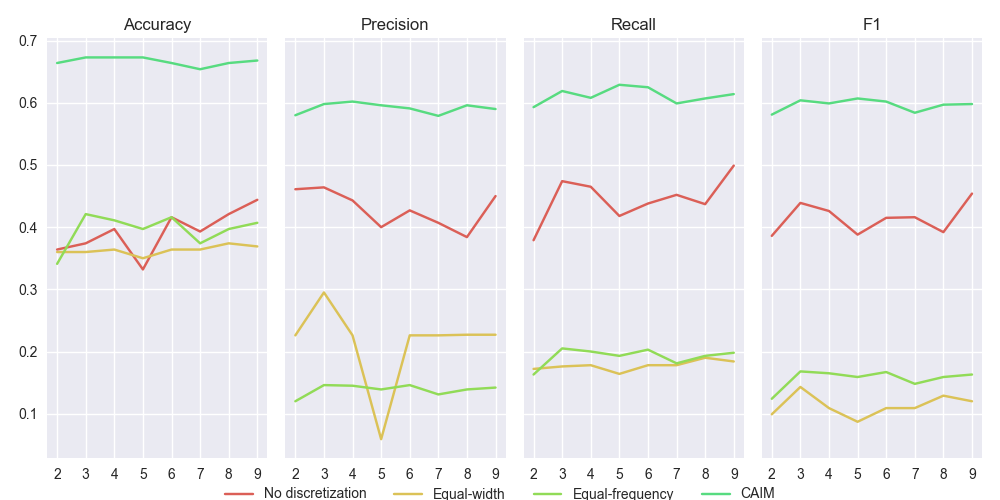
\includegraphics[width=\textwidth]{img/cv_scores_stratifiedkfold/scoring_stratifiedkfold_glass.png}
    \caption{Wykresy wartości metryk dla zbioru "Glass" -- kroswalidacja stratyfikowana.}
\end{figure}

Poprawę jakości uczenia klasyfikatora przy kroswalidacji stratyfikowanej, można zaobserwować również
na przykładzie macierzy konfuzji (wybranej dla parametru $K = 5$). Wartości wzdłuż przekątnej ("prawidłowe"
klasyfikacje) są wyraźnie wyższe i zatem lepsze.

\begin{figure}[H]
\center
    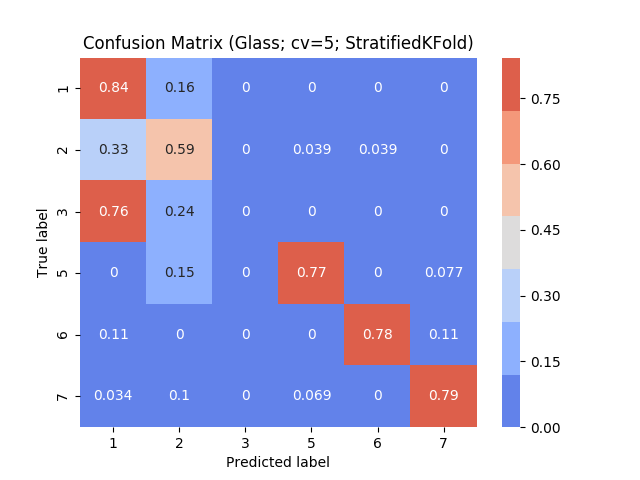
\includegraphics[width=0.6\textwidth]{img/conf_matrices/cm_Glass_cv5_StratifiedKFold.png}
    \caption{Macierz konfuzji dla najlepszej wartości F1 -- kroswalidacja stratyfikowana.}
\end{figure}


\begin{table}[H]
\center
    \caption{Wartości metryk dla zbioru "Glass" -- kroswalidacja stratyfikowana.}
    \begin{tabular}{|c|c|c|c|c|c|c|c|c|c|}
        \hline
        \multirow{2}{*}{\textbf{Metoda dyskr.}} & \multirow{2}{*}{\textbf{Metryka}} & \multicolumn{8}{|c|}{\textbf{CV}} \\ \cline{3-10}
                        &  & 2 & 3 & 4 & 5 & 6 & 7 & 8 & 9 \\ \hline
        \multirow{4}{*}{\textit{Brak}}  & Accuracy & 0.364 & 0.374 & 0.397 & 0.332 & 0.416 & 0.393 & 0.421 & 0.444 \\ \cline{2-10}
                                         & Precision & 0.461 & 0.464 & 0.443 & 0.4 & 0.427 & 0.407 & 0.384 & 0.45 \\ \cline{2-10}
                                         & Recall & 0.379 & 0.474 & 0.465 & 0.418 & 0.438 & 0.452 & 0.437 & 0.499 \\ \cline{2-10}
                                         & F1 & 0.386 & 0.439 & 0.426 & 0.388 & 0.415 & 0.416 & 0.392 & 0.454 \\ \hline \hline


        \multirow{4}{*}{\textit{Equal-width}}  & Accuracy & 0.36 & 0.36 & 0.364 & 0.35 & 0.364 & 0.364 & 0.374 & 0.369 \\ \cline{2-10}
                                             & Precision & 0.226 & 0.295 & 0.226 & 0.059 & 0.226 & 0.226 & 0.227 & 0.227 \\ \cline{2-10}
                                             & Recall & 0.172 & 0.176 & 0.178 & 0.164 & 0.178 & 0.178 & 0.19 & 0.184 \\ \cline{2-10}
                                             & F1 & 0.099 & 0.143 & 0.109 & 0.087 & 0.109 & 0.109 & 0.129 & 0.12 \\ \hline \hline


        \multirow{4}{*}{\textit{Equal-freq}}  & Accuracy & 0.341 & 0.421 & 0.411 & 0.397 & 0.416 & 0.374 & 0.397 & 0.407 \\ \cline{2-10}
                                             & Precision & 0.12 & 0.146 & 0.145 & 0.139 & 0.146 & 0.131 & 0.139 & 0.142 \\ \cline{2-10}
                                             & Recall & 0.163 & 0.205 & 0.2 & 0.193 & 0.203 & 0.181 & 0.193 & 0.198 \\ \cline{2-10}
                                             & F1 & 0.124 & 0.168 & 0.165 & 0.159 & 0.167 & 0.148 & 0.159 & 0.163 \\ \hline \hline


        \multirow{4}{*}{\textit{CAIM}}  & Accuracy & 0.664 & 0.673 & 0.673 & 0.673 & 0.664 & 0.654 & 0.664 & 0.668 \\ \cline{2-10}
                                     & Precision & 0.58 & 0.598 & 0.602 & 0.596 & 0.591 & 0.579 & 0.596 & 0.59 \\ \cline{2-10}
                                     & Recall & 0.593 & 0.619 & 0.608 & 0.629 & 0.625 & 0.599 & 0.607 & 0.614 \\ \cline{2-10}
                                     & F1 & 0.581 & 0.604 & 0.599 & 0.607 & 0.602 & 0.584 & 0.597 & 0.598 \\ \hline \hline

            \hline
    \end{tabular}
\end{table}
